\section{Repair regions with noisy verification}
\label{sec:geometry}
\subsection{Affine pieces determine a component bound}
Return to a binary environment and a fixed visible state. Before repair, any
finite collection of information and control actions is allowed, with
belief-independent physical availability as in Section~\ref{sec:model}.
Consider one specified deterministic, irreversible repair $u$. Following $u$,
there are no further intervention choices: a fixed task policy is used and a
passive observation transcript $Z$ is obtained before the terminal declaration.
Let $q_i(z)$ be its finite distribution under environment $i$. Suppose the
repaired representation has opposite adequacy labels in the two environments,
terminal error costs are symmetric $\lambda$, and the expected nonterminal
cost of this repair plan is affine, $a_u(p)$.

The repair-now value is then
\begin{equation}
R_u(p)=a_u(p)+\lambda\sum_z\min\{(1-p)q_0(z),\,p q_1(z)\}.
\label{eq:repairrisk}
\end{equation}
The sum uses joint prior--transcript masses. No posterior normalization is
needed. Its interior breakpoints are the distinct values
\begin{equation}
\mathcal B_u=
\left\{\frac{q_0(z)}{q_0(z)+q_1(z)}:
q_0(z)q_1(z)>0\right\}.
\end{equation}
If there are $m_u$ distinct breakpoints, there are at most $m_u+1$ affine pieces.
Transcripts possible in only one environment contribute zero decision risk.

\begin{theorem}[A repair-region component bound]
\label{thm:geometry}
Under the preceding assumptions, the set of priors where repair $u$ is weakly
optimal is the union of at most $m_u+1$ closed intervals, allowing empty intervals
and singletons. On every affine piece of $R_u$, its intersection with the repair
region is an interval. If the post-repair transcript is uninformative, the
repair region has at most two connected components.
\end{theorem}
\begin{proof}
Let $C_u(p)$ be the optimal value among all policy trees whose first action is
not $u$. It is a minimum of finitely many affine functions of $p$ by
Proposition~\ref{prop:standard}; hence it is concave and continuous.
The repair region is $\{p:R_u(p)\le C_u(p)\}$. On any closed piece where $R_u$
is affine, $C_u-R_u$ is concave, and its nonnegative superlevel set is convex.
A closed convex subset of an interval is an interval, a singleton, or empty.
Taking the union over at most $m_u+1$ pieces proves the bound. If $q_0=q_1$,
the decision risk is $\lambda\min(p,1-p)$ with the single breakpoint $1/2$.
\end{proof}

The result applies regardless of the complexity of the optimal \emph{pre-repair}
continuation. It needs no TP2 assumption on verification. It does need the
specified passive continuation after repair; allowing subsequent controlled
repairs replaces \eqref{eq:repairrisk} by a more complicated piecewise-linear
continuation value and does not preserve the two-component bound automatically.
The bound is about components of one action's optimality region, not the
piece count of the entire optimal policy.

\begin{corollary}[Independent binary observations after repair]
\label{cor:counts}
If repair is followed by $n$ independent Bernoulli observations with distinct
full-support success probabilities in the two environments, then $m_u\le n+1$
and the repair region has at most $n+2$ connected components.
\end{corollary}
\begin{proof}
The likelihood ratio of a transcript depends only on its number of successes,
which takes $n+1$ values. Apply Theorem~\ref{thm:geometry}.
\end{proof}
This is an upper bound, not a claim that every number of components is
attainable for every channel. More informative observations improve optimal
value under the conditions in Section~\ref{sec:information}, but component counts
and region inclusion need not be monotone.

\subsection{A sharp two-region example with a TP2 channel}
\label{sec:counter}
Consider one remaining round, symmetric terminal cost $\lambda=2$, old task
losses $(0,2)$, and repaired task losses $(1/5,0)$. Repair is deterministic,
irreversible, costs $1/10$, and yields no environment information. Verification
costs $1/2$, replaces that round's ordinary task (zero additional task loss),
leaves the representation unchanged, and observes a binary signal with
\begin{equation}
P(Y=1\mid I=0)=\frac15,\qquad
P(Y=1\mid I=1)=\frac45.
\end{equation}
Both observation distributions have full support. The channel matrix with
ordered states and signals has determinant $3/5>0$ and is TP2.
The three action values are
\begin{align}
K(p)&=2p+2\min(p,1-p),\\
R(p)&=\frac1{10}+\frac{1-p}{5}+2\min(p,1-p),\\
B(p)&=\frac12+2\min\left\{p,\frac15,1-p\right\}.
\label{eq:countervalues}
\end{align}
The verification formula follows by summing the smaller joint mass for each
signal. All three actions share the same terminal loss contract.

\begin{theorem}[Disconnected repair and strict early intervention]
\label{thm:counter}
In this full-support noisy-verification instance, the weak repair region is
\begin{equation}
\mathcal R=
\left[\frac3{22},\frac13\right]\ \cup\
\left[\frac7{11},1\right].
\label{eq:tworegions}
\end{equation}
The keep region is $[0,3/22]$ and the verify region is $[1/3,7/11]$, with
shared endpoints denoting ties. In particular, TP2 verification alone does not
guarantee a single repair interval. For every
$p\in(3/22,1/3)$, repair is the unique optimal action while the immediate
declaration benchmark prefers adequate.
\end{theorem}
\begin{proof}
For $p\le1/2$, $R(p)=3/10+9p/5$; for $p\ge1/2$,
$R(p)=23/10-11p/5$. Comparing $R$ and $K$ gives $p\ge3/22$.
The verification value equals $1/2+2p$ on $[0,1/5]$, $9/10$ on
$[1/5,4/5]$, and $5/2-2p$ on $[4/5,1]$.
On the middle interval, $R\le B$ holds for $p\le1/3$ or $p\ge7/11$.
On the two exterior intervals, $R<B$. Combining the inequalities gives
\eqref{eq:tworegions}; comparing $K$ and $B$ on the remaining pieces gives the
other regions. Strict inequalities hold in the stated interiors. Finally
$p<1/2=p_{\dec}$ throughout $(3/22,1/3)$.
\end{proof}

At $p=1/4$, the three costs are $K=1$, $B=9/10$, and $R=3/4$.
The joint controller repairs, while the declaration gate permits only keep or
verify and chooses verify. Its exact extra cost is $3/20$.
At $p=1/2$, verification is preferable; at sufficiently high $p$, repair is
again preferable. A single threshold therefore misses an optimal repair region
even though the pairwise repair--keep comparison has a threshold.

\begin{figure}[ht]
\centering
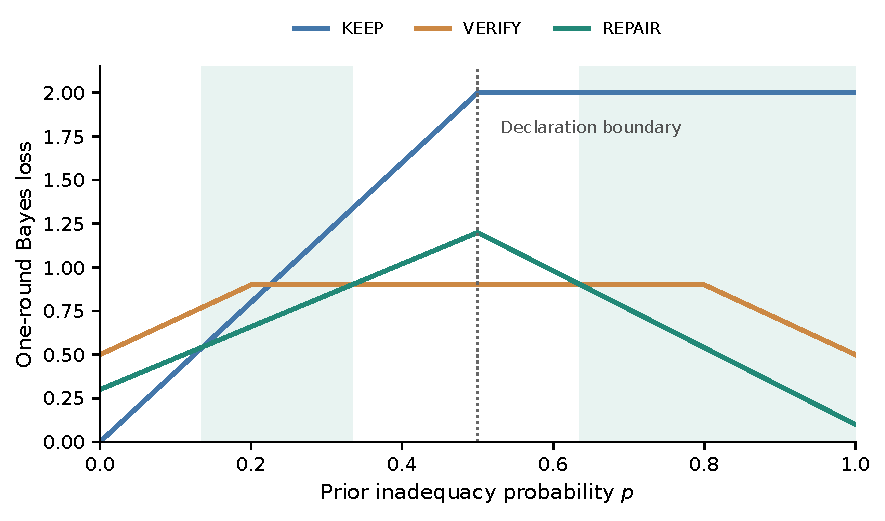
\includegraphics[width=.92\linewidth]{figures/disconnected_region.pdf}
\caption{Exact one-round action values. Shading marks the two repair intervals.
The dotted line is the declaration boundary, not an action constraint for the
joint controller. The lower repair interval lies entirely below that boundary.}
\label{fig:counter}
\end{figure}

\subsection{Robustness beyond one parameter point}
\begin{proposition}[Finite-horizon perturbation certificate]
\label{prop:robust}
Consider two models with the same finite environment, states, actions,
observation alphabet, and terminal decision sets. Suppose corresponding kernel
rows differ by at most $\epsilon_Q$ in total variation, stage costs differ by
at most $\epsilon_\ell$, and terminal costs differ by at most $\epsilon_L$.
Both stage and terminal costs are bounded by $L_{\max}$ and $L_B$, respectively.
For any fixed horizon-$h$ policy tree, and hence for an optimal value or a
root-action-constrained optimal value, the absolute value difference is at most
\begin{equation}
\mathcal E_h=
h\epsilon_\ell+\epsilon_L+
\epsilon_Q\left\{L_{\max}\frac{h(h+1)}2+hL_B\right\}.
\label{eq:robustbound}
\end{equation}
A unique action with gap $g>2\mathcal E_h$ remains uniquely optimal.
\end{proposition}
\begin{proof}
Condition on the same environment and couple corresponding observable events
maximally while histories agree. The probability that histories differ by the
end of round $t$ is at most $t\epsilon_Q$. The round-$t$ loss difference is
bounded by $\epsilon_\ell+tL_{\max}\epsilon_Q$ for $t=1,\ldots,h$; the terminal
difference is at most $\epsilon_L+hL_B\epsilon_Q$. Summation gives
\eqref{eq:robustbound}. The bound is uniform over policy trees. Taking minima
over the same feasible set preserves it, including when the first action is
fixed. Two action values can move toward one another by at most
$2\mathcal E_h$.
\end{proof}
At $p=1/4$, the strict repair margin is $3/20$. Continuity or the explicit bound
therefore gives a neighborhood of costs and full-support channel probabilities
where early repair remains uniquely optimal. The prior is also separated from
the declaration boundary. Thus the phenomenon holds on a nonempty open
parameter set, not only at a rational point. This perturbation statement keeps
physical action sets fixed; it does not assert continuity across arbitrary
changes in belief-dependent gates.
